% Results. Every number is a macro from paper/numbers.tex (scripts/make_tables.py).
% Convention: P_K = probability that the best of K samples is an exact ground state; "scenario level" = paired over
% the \NScen held-out scenarios (seed means first); "group level" = one value per structural group (n = \NGroupsGL).
% Full tables moved to paper/supplement.tex: main table (S3), 22 qubits (S4), band-share fits (S5), wrong-pin
% census (S6), robustness (S7), out of distribution (S8), classical samplers (S9); figures S1 (eps), S2 (classical).
\section{Results}
\label{sec:results}

\subsection{Wrong pins degrade sampling with a dose--response}
\label{sec:res-pins}

\paragraph{Unit commitment} At $n=\NLtwo$, $p=1$ and $\varepsilon=\EpsMain$, the learned start C-milp reaches $P_{\KMax}=\PgndCmilp$ \PgndCICmilp\ and the LP relaxation (D) \PgndD\ \PgndCID. The LP's deficit is confined to instances where it pins several bits to values the ground state does not take, and it grows with their number (Table~\ref{tab:dose}). C-milp $-$ D is $\DoseLtwoLow$ for the \DoseLtwoLowN\ scenarios with 0--1 wrong pins, $\DoseLtwoTwo$ for the \DoseLtwoTwoN\ with exactly two, and $\DoseLtwoThree$ for the \DoseLtwoThreeN\ with three or more. The same pattern holds at \NLfour\ qubits at both operating points: with three or more wrong pins C-milp leads by \DoseLfourFrzThree\ and \DoseLfourOwnThree, with intervals clear of zero; with 0--1 the LP is slightly better (\DoseLfourFrzLow\ and \DoseLfourOwnLow, intervals including zero). The learned start pins far fewer bits wrongly: \LfourOwnWrongCmilp\ per instance at L4's own point, against \LfourOwnWrongD\ for the LP.

The wrong pins fall on small, expensive marginal units. In the L4 census the per-block wrong-pin rate has Spearman correlation \ConcCapLfour\ with capacity and \ConcRankLfour\ with merit-order rank; the large, cheap units are never wrongly pinned.

\paragraph{MaxCut} On UC the dose comes with the source. On MaxCut we set it by hand (Table~\ref{tab:maxcut}). At $\varepsilon=\MCDoseEps$, a start with up to two wrongly pinned vertices returns a maximum cut with probability \MCDoseTwoMin\ at every size. With three it is \MCDoseThreeMin--\MCDoseThreeMax\ and with four \MCDoseFourMin--\MCDoseFourMax. Goemans--Williamson cuts, binned by their own wrong pins at $\varepsilon=\EpsMain$, follow the same curve: \MCGWPinsLow\ with at most two, \MCGWPinsFour\ with four and \MCGWPinsFive\ with five. A larger $\varepsilon$ flattens the curve, as on UC. The mechanism therefore needs neither a relaxation nor the UC encoding.

\begin{table}[t]
\centering
\caption{Dose--response on UC: $P_{\KMax}$ by the number of bits the LP pins wrongly ($p=1$, $\varepsilon=\EpsMain$). Inst.: scenarios (L2) or structures (L4) in the bin; 95\% $t$-interval of the paired difference.}
\label{tab:dose}
\scriptsize
\setlength{\tabcolsep}{2.5pt}
\begin{tabular}{lcccc}
\toprule
System, LP wrong pins & Inst. & C-milp & D (LP) & C-milp $-$ D [95\% CI] \\
\midrule
L2 ($n{=}16$), 0--1 & 20 & 1.000 & 1.000 & 0.000 \ensuremath{[0.000,\,0.000]} \\
L2 ($n{=}16$), 2 & 5 & 0.991 & 0.728 & \ensuremath{+0.263} \ensuremath{[-0.037,\,+0.562]} \\
L2 ($n{=}16$), $\geq$3 & 5 & 0.948 & 0.169 & \ensuremath{+0.780} \ensuremath{[+0.557,\,+1.002]} \\
\midrule
L4 frozen ($n{=}22$), 0--1 & 5 & 0.906 & 1.000 & \ensuremath{-0.094} \ensuremath{[-0.267,\,+0.079]} \\
L4 frozen ($n{=}22$), 2 & 5 & 0.850 & 0.848 & \ensuremath{+0.002} \ensuremath{[-0.370,\,+0.374]} \\
L4 frozen ($n{=}22$), $\geq$3 & 10 & 0.516 & 0.054 & \ensuremath{+0.462} \ensuremath{[+0.251,\,+0.673]} \\
\midrule
L4 own point ($n{=}22$), 0--1 & 7 & 0.930 & 0.999 & \ensuremath{-0.069} \ensuremath{[-0.173,\,+0.035]} \\
L4 own point ($n{=}22$), 2 & 4 & 0.993 & 0.839 & \ensuremath{+0.154} \ensuremath{[-0.115,\,+0.424]} \\
L4 own point ($n{=}22$), $\geq$3 & 9 & 0.556 & 0.057 & \ensuremath{+0.498} \ensuremath{[+0.295,\,+0.702]} \\
\bottomrule
\end{tabular}

\end{table}

\begin{table}[t]
\centering
\caption{3-regular MaxCut, $p=1$, \MCGraphs\ graphs per size. Cold: $P_{\KMax}$ of the cold start. Columns 3--5: $P_{\KMax}$ of the badly pinned starts by wrong pins ($\varepsilon=\MCDoseEps$). Columns 6--8: $R^2$ of the logistic fit of $P_{\KMax}$ on overlap, on overlap and band mass, and of the UC curve applied unchanged. Last two: graphs on which the rule picks the best source ($\varepsilon=\EpsMain$; graphs where all sources tie are left out).}
\label{tab:maxcut}
\scriptsize
\setlength{\tabcolsep}{2.5pt}
\begin{tabular}{c|c|ccc|ccc|cc}
\toprule
$n$ & Cold & $\leq$2 & 3 & 4 & Ov. & +Band & UC curve & Ov. & Band \\
\midrule
12 & 1.000 & 1.00 & 0.83 & 0.35 & 0.86 & 0.86 & \ensuremath{-0.07} & 24/24 & 0/24 \\
16 & 0.998 & 1.00 & 0.81 & 0.24 & 0.84 & 0.90 & \ensuremath{+0.26} & 29/29 & 20/29 \\
20 & 0.881 & 1.00 & 0.78 & 0.23 & 0.72 & 0.86 & \ensuremath{-0.02} & 30/30 & 10/30 \\
\bottomrule
\end{tabular}

\end{table}

\subsection{The LP's wrong pins grow with problem size}
\label{sec:res-size}

Refining the fleet adds exactly the small marginal units that attract wrong pins, so a size study along granularity alone would be circular. We separated two axes (Fig.~\ref{fig:size}; Supplementary Table~S6): the horizon at fixed blocks, and granularity at $T=\NHoursMain$. Each cell used \NCensus\ paired demand draws at its own calibrated point, with no QAOA.

Along the horizon no new units appear, yet the LP's wrong pins grow linearly with the number of hours: each added variable adds $\SlopeHorLPLzero$ \SlopeHorLPLzeroCI\ wrongly pinned bits at L0, $\SlopeHorLPLone$ at L1 and $\SlopeHorLPLtwo$ at L2. The fraction of draws with two or more wrong pins at L0 rises from \FracTwoLzeroTOne\ at $T=1$ to \FracTwoLzeroTFour\ at $T=4$. Along granularity they grow at $\SlopeGranLP$ \SlopeGranLPCI\ per added variable.

The learned start's wrong pins grow too, but \SlopeRatioMin--\SlopeRatioMax\ times more slowly: a GCN trained at each horizon gains $\SlopeHorGCNLzero$, $\SlopeHorGCNLone$ and $\SlopeHorGCNLtwo$ per variable at L0, L1 and L2.

\begin{figure*}[t]
\centering
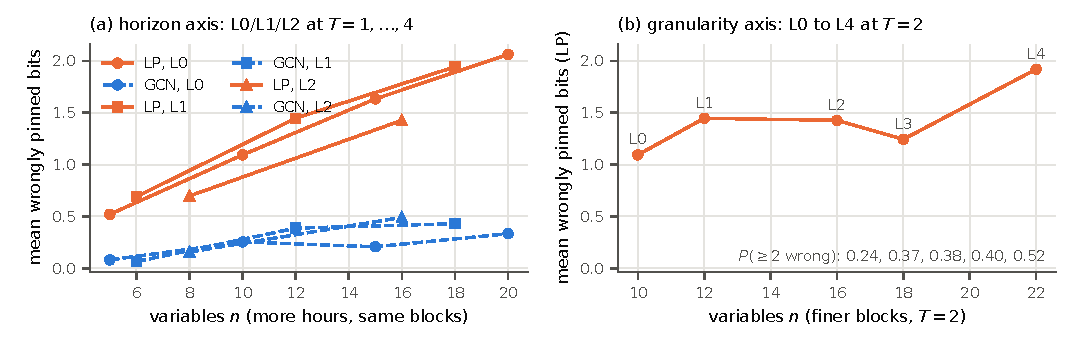
\includegraphics[width=0.72\textwidth]{figures/fig_size.pdf}
\caption{Mean wrongly pinned bits against problem size, \NCensus\ paired demand draws per cell, each cell at its own calibrated point. (a) Horizon at fixed granularity: the LP (solid) and a GCN trained at each horizon (dashed). (b) Granularity at $T=\NHoursMain$, L0--L4 (LP).}
\label{fig:size}
\end{figure*}

\subsection{Band share explains sampling on UC, not on MaxCut}
\label{sec:res-band}

\paragraph{The fit on UC} We pooled every $p=1$ run of the $\varepsilon$ sweep with nonzero overlap (all arms and all $\varepsilon$) and fitted $P_{\KMax}$ by logistic least squares (Fig.~\ref{fig:bandshare}; Supplementary Table~S5). $\log_{10}$ overlap alone gives $R^2=\BSRtwoOverlap$, and the arms separate: the per-arm mean residuals span \BSSpreadOverlap. Adding the band mass $m_5$ gives $R^2=\BSRtwoBand$, cuts the residual spread to \BSSpreadBand, and leaves nothing for arm-specific intercepts ($\Delta R^2=\BSdRtwoBand$). The coefficient on $\log_{10}m_5$ is \emph{negative} (\BSCoefBand, against \BSCoefOverlap\ on $\log_{10}$ overlap): at fixed overlap, more initial mass on other near-ground states means lower ground-state sampling.

\paragraph{Held-out checks on UC} Fitted only on the non-learned runs, overlap alone under-predicts the learned arms by \BSHeldOutOverlapMin--\BSHeldOutOverlapMax; overlap plus band mass predicts them within \BSHeldOutBandMax. Leaving out one structural group at a time, the cross-validated $R^2$ is \BSLogoOverlap\ for overlap alone and \BSLogoBand\ with band mass. At L4 the refit gives \BSLfourBand\ (overlap alone: \BSLfourOverlap), and the L2 curve applied \emph{unchanged} to L4 gives $R^2=\BSTransferBand$, against \BSTransferOverlap\ for the transferred overlap-only curve.

\paragraph{No transfer to MaxCut} The same curve applied unchanged to MaxCut fails: $R^2=\MCTransferTwelve$, \MCTransferSixteen\ and \MCTransferTwenty\ at $n=\MCSizeTwelve$, \MCSizeSixteen\ and \MCSizeTwenty\ (Table~\ref{tab:maxcut}). Refitted there, overlap alone already gives \MCOvTwelve, \MCOvSixteen\ and \MCOvTwenty, and band mass raises this to \MCBandTwelve, \MCBandSixteen\ and \MCBandTwenty, with source-specific residuals remaining. At $n=\MCSizeTwelve$ the band holds only the maximum cuts, so band share and overlap coincide. Band density does not explain the difference: across the \BDInstances\ instances of both classes it correlates with the improvement from the band (rank correlation \BDPooled), but within classes it does not (\BDWithin). Band share is a diagnostic for unit commitment; computing it needs the full spectrum.

\begin{figure*}[t]
\centering
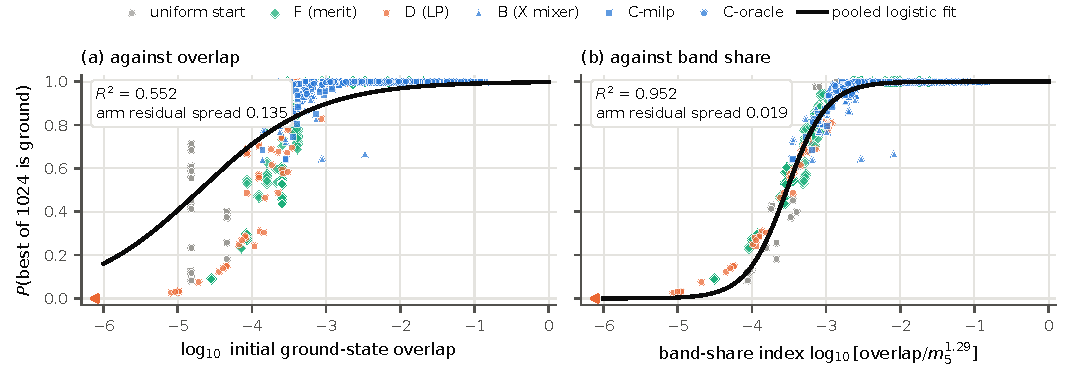
\includegraphics[width=0.72\textwidth]{figures/fig_bandshare.pdf}
\caption{UC, L2, $p=1$: $P_{\KMax}$ against (a) the initial ground-state overlap and (b) the band-share index $\log_{10}(\mathrm{overlap}/m_5^{k})$, $k=\BSExponent$ fitted. Points: arm $\times$ $\varepsilon$ $\times$ scenario means; curves: one logistic fit pooled over all arms and $\varepsilon$. On overlap the arms separate; on band share they collapse onto one curve.}
\label{fig:bandshare}
\end{figure*}

\subsection{Overlap ranks sources well and chooses $\varepsilon$ badly}
\label{sec:res-eps}

\paragraph{Ranking sources} Earlier work ranks warm starts by depth-zero quantities: initial overlap and initial approximation ratio~\cite{bhattacharyya2025qubo}. As a rule for picking the source with the highest $P_{\KMax}$ at $\varepsilon=\EpsMain$, overlap is right in \RKUCSixteenOv\ of \RKUCSixteenN\ UC instances at \NLtwo\ qubits and \RKUCTwentyTwoOv\ of \RKUCTwentyTwoN\ at \NLfour, and on every MaxCut graph where sources differ (Table~\ref{tab:maxcut}). Band share matches it on UC (\RKUCSixteenBand\ and \RKUCTwentyTwoBand) and is worse on MaxCut. The initial approximation ratio is right in only \RKUCSixteenRatio\ and \RKUCTwentyTwoRatio.

\paragraph{Choosing $\varepsilon$} A wrong $\varepsilon$ is expensive for the LP and nearly free for the learned starts (Table~\ref{tab:eps}). Measured from an arm's best $\varepsilon$ at the group level, the LP's regret is \RegretEpsFiveD\ \RegretEpsFiveDCI\ at $\varepsilon=\EpsSecond$ and \RegretEpsZeroD\ at $\varepsilon=0$, where a wrongly pinned bit can never flip. For the learned starts it is at most \RegretMaxCmilp\ (C-milp) and \RegretMaxCoracle\ (C-oracle) anywhere in $0\leq\varepsilon\leq\RegretRange$.

Choosing $\varepsilon$ per instance by maximum overlap does not remove this cost for heuristic sources, because overlap favours small $\varepsilon$. Against each instance's own best $\varepsilon$, the LP loses \ERDOvSixteen\ on average (worst instance \ERDOvWorstSixteen) and merit order \ERFOvSixteen\ (\ERFOvWorstSixteen) at \NLtwo\ qubits, and \ERDOvTwentyTwo\ (\ERDOvWorstTwentyTwo) and \ERFOvTwentyTwo\ (\ERFOvWorstTwentyTwo) at \NLfour, where the choice is between two values only. Choosing by band share loses at most \ERBandMeanMax\ on average and \ERBandWorstMax\ on one instance. For the learned starts every rule is within \ERLearnedMax\ of the best.

\begin{table*}[t]
\centering
\caption{Regularisation on UC. Each arm at its best $\varepsilon^\star$ (maximising scenario-mean $P_{\KMax}$; $\varepsilon=\EpsMax$ excluded); L2, $p=1$, \NScen\ scenarios $\times$ \NSeedsSweep\ seeds. $g$: final gain. Regret: drop in group-level $P_{\KMax}$ from $\varepsilon^\star$. Last three columns: the LP (at its own $\varepsilon^\star$) minus the arm, paired over scenarios and over the \NGroupsGL\ structural groups (95\% $t$-intervals), and group-fold cross-validated over \NSplits\ splits (mean; share of splits in which D is worse).}
\label{tab:eps}
\scriptsize
\setlength{\tabcolsep}{2.5pt}
\resizebox{\textwidth}{!}{\begin{tabular}{lcccccccccc}
\toprule
Arm & $\varepsilon^\star$ & $P_{\KMax}$ at $\varepsilon^\star$ [95\% CI] & $g$ at $\varepsilon^\star$ & $g$ at $\EpsMain$ & Regret $\varepsilon{=}0$ & Regret $\varepsilon{=}\EpsSecond$ & D $-$ arm, scenarios & D $-$ arm, GL groups & D $-$ arm, group CV \\
\midrule
C-oracle (GCN) & 0.1 & 1.000 \ensuremath{[1.000,\,1.000]} & 0.936 & 0.936 & 0.000 & 0.000 & \ensuremath{-0.100} \ensuremath{[-0.164,\,-0.036]} & \ensuremath{-0.083} \ensuremath{[-0.164,\,-0.003]} & \ensuremath{-0.094} (100\%) \\
C-milp (GCN) & 0.15 & 0.991 \ensuremath{[0.978,\,1.005]} & 0.924 & 0.936 & 0.018 & 0.010 & \ensuremath{-0.092} \ensuremath{[-0.153,\,-0.031]} & \ensuremath{-0.069} \ensuremath{[-0.140,\,+0.003]} & \ensuremath{-0.070} (96\%) \\
B (GCN, X mixer) & 0.15 & 0.994 \ensuremath{[0.985,\,1.003]} & 0.914 & 0.927 & 0.018 & 0.007 & \ensuremath{-0.094} \ensuremath{[-0.156,\,-0.032]} & \ensuremath{-0.073} \ensuremath{[-0.147,\,+0.001]} & \ensuremath{-0.079} (98\%) \\
F (merit order) & 0.25 & 0.863 \ensuremath{[0.811,\,0.915]} & 0.912 & 0.935 & 0.197 & 0.197 & \ensuremath{+0.037} \ensuremath{[-0.026,\,+0.099]} & \ensuremath{+0.047} \ensuremath{[-0.028,\,+0.122]} & \ensuremath{+0.036} (20\%) \\
\midrule
D (LP) & 0.25 & 0.900 \ensuremath{[0.836,\,0.964]} & 0.905 & 0.946 & 0.917 & 0.122 & -- & -- & -- \\
\bottomrule
\end{tabular}
}
\end{table*}

\subsection{The unit-commitment study}
\label{sec:res-arms}

\paragraph{Sources at $\varepsilon=\EpsMain$} Over \NScen\ held-out scenarios $\times$ \NSeedsMain\ seeds (Supplementary Table~S3), C-milp reaches $P_{\KMax}=\PgndCmilp$ and C-oracle \PgndCoracle; the LP reaches \PgndD, merit order (F) \PgndF, the cold start (A) \PgndA\ and the random control (E) \PgndE. Paired over scenarios, C-milp $-$ D $=\CmilpMinusD$ \CmilpMinusDCI\ (C-milp ahead in \CmilpMinusDW\ of \CmilpMinusDN), C-milp $-$ F $=\CmilpMinusF$ \CmilpMinusFCI\ and C-milp $-$ A $=\CmilpMinusA$ \CmilpMinusACI.

At the group level ($n=\NGroupsGL$), C-milp $-$ F and C-milp $-$ A keep intervals clear of zero (\CmilpMinusFGL\ \CmilpMinusFGLCI\ and \CmilpMinusAGL\ \CmilpMinusAGLCI). C-milp $-$ D is \CmilpMinusDGL\ \CmilpMinusDGLCI, an interval that touches zero: the effect against D is large in a minority of structures and zero in the rest (Section~\ref{sec:res-pins}).

Exact ground-state labels buy nothing over MILP labels (C-oracle $-$ C-milp $=\CoracleMinusCmilp$ \CoracleMinusCmilpCI). The learned state with the $X$ mixer (B) ties C-milp on $P_{\KMax}$ but is worse on single-shot $P_1$ ($\PoneBMinusCmilp$ \PoneBMinusCmilpCI). The random control is worse than starting cold (E $-$ A $=\EMinusA$ \EMinusACI). Depth barely helps the warm arms: from $p=1$ to $p=3$ C-milp moves from \PgndCmilp\ to \PgndPthreeCmilp\ and D from \PgndD\ to \PgndPthreeD.

\label{sec:res-tuned}
\paragraph{The advantage survives tuning the LP} At its own best $\varepsilon=\BestEpsD$ the LP reaches \PgndBestD\ \PgndBestCID\ (Table~\ref{tab:eps}). Paired, D $-$ C-oracle $=\BestDMinusCoracle$ \BestDMinusCoracleCI\ (group level \BestDMinusCoracleGL\ \BestDMinusCoracleGLCI), and D $-$ C-milp $=\BestDMinusCmilp$ \BestDMinusCmilpCI. At the group level the latter is \BestDMinusCmilpGL\ \BestDMinusCmilpGLCI, so granting D its in-sample best $\varepsilon$ leaves the group-level gap to C-milp borderline.

Choosing $\varepsilon$ on the scenarios it is evaluated on flatters the arm whose optimum is noisiest. Our primary numbers therefore choose $\varepsilon$ on half of the structural groups and evaluate on the other half, over \NSplits\ random splits: D $-$ C-oracle $=\CVDMinusCoracle$ (D worse in \CVDMinusCoracleWorse\% of splits), D $-$ C-milp $=\CVDMinusCmilp$ (\CVDMinusCmilpWorse\%), and D $-$ F $=\CVDMinusF$, so at its best the LP is indistinguishable from merit order.

\paragraph{Approximation ratio and sampling disagree} At $\varepsilon=\EpsMain$ the LP has the highest final gain of any arm (\GfinalD, against \GfinalCoracle\ for C-oracle), higher than C-oracle in all \GfinalCoracleMinusDL\ scenarios, while sampling the ground state less reliably in \CoracleMinusDW\ of \CoracleMinusDN. At each arm's own best $\varepsilon$ the gain order reverses, because the LP's sampling optimum lies at a larger $\varepsilon$, which moves the initial state towards uniform: the LP gives up gain to dilute its wrongly pinned bits.

\paragraph{At \NLfour\ qubits} Over \LfourNStruct\ structurally distinct L4 instances $\times$ \NSeedsLfour\ seeds at L4's own operating point (Supplementary Table~S4), C-milp $-$ D $=\LfourOwnCmilpMinusDTen$ \LfourOwnCmilpMinusDTenCI\ per structure at $\varepsilon=\EpsMain$ (C-milp ahead in \LfourOwnCmilpMinusDTenW\ of \LfourNStruct), and \LfourOwnCmilpMinusDTenRw\ \LfourOwnCmilpMinusDTenRwCI\ reweighted to the demand distribution. At the frozen point it is \LfourFrzCmilpMinusDTen\ \LfourFrzCmilpMinusDTenCI; the paired change between the two points is \LfourChangeTen\ \LfourChangeTenCI, consistent with zero though wide. Every arm does worse than at \NLtwo\ qubits: C-milp reaches \LfourOwnPgndCmilp, D \LfourOwnPgndD\ and the cold start \LfourOwnPgndA.

\label{sec:res-robust}
\paragraph{Robustness} With \ShotsMin-shot expectation estimates (Supplementary Table~S7), C-milp loses \ShotLossCmilp\ in $P_{\KMax}$, the LP \ShotLossD, the cold start \ShotLossA\ and merit order \ShotLossF. The learned start's advantage over the LP does not change significantly (\ShotAdvChange\ \ShotAdvChangeCI). Under shot noise COBYLA stops early, so this is a lightly optimised regime. Nelder--Mead with exact expectations gives C-milp $-$ D $=\NMCmilpMinusD$ \NMCmilpMinusDCI, against \ExactThreeSeedCmilpMinusD\ with COBYLA on the same runs.

\subsection{Negative results}
\label{sec:res-neg}

\paragraph{The learned start fails below its training range} We applied the unchanged L2 GCN to new conditions, \OODNScen\ scenarios $\times$ \NSeedsOOD\ seeds per test set (Supplementary Table~S8). Below the training demand range the learned start is worse than the LP: its wrong pins rise to \OODLowWrongC\ per instance (LP \OODLowWrongD), and its $P_{\KMax}$ falls to \OODLowC\ against \OODLowD: C-milp $-$ D $=\OODLowDiff$ \OODLowDiffCI, with C-milp behind in \OODLowDiffL\ of \OODNScen\ scenarios. With a changed hourly profile it falls to LP level (flat: \OODFlatC\ against \OODFlatD; reversed: \OODRevC\ against \OODRevD). A forced outage, which changes the graph, does not break it: it keeps $P_{\KMax}$ between \OODOutMin\ and \OODOutMax, at or above the LP. The LP has no training distribution to fall out of, which is a genuine advantage.

\paragraph{All warm starts are equivalent on cost} The learned starts sample the ground state more often, but their best-of-\KMax operating cost is no better than the LP's. At L2, C-milp $-$ D in repaired cost gap is \GapCmilpMinusD\ percentage points \GapCmilpMinusDCI\ at the scenario level and \GapCmilpMinusDGL\ \GapCmilpMinusDGLCI\ at the group level; at L4 it is \LfourFrzGapCmilpMinusD\ \LfourFrzGapCmilpMinusDCI\ (frozen point) and \LfourOwnGapCmilpMinusD\ \LfourOwnGapCmilpMinusDCI\ (own point). When the LP misses the ground state, it lands on a near-optimal adequate schedule.

\paragraph{A classical sampler solves these instances in milliseconds} Simulated annealing on the identical QUBO, compiled, with every returned state checked against the brute-force energy vector (Supplementary Table~S9), reaches $P(\text{ground})=\SAPgndLtwoEFive$ in \SAmsLtwoEFive\,ms at $n=\NLtwo$, against QAOA C-milp's \QAOAPgndLtwo\ in \QAOATimeLtwo\,s of simulation, and \SAPgndLfourESix\ in \SAmsLfourESix\,ms at $n=\NLfour$, against \QAOAPgndLfour\ in \QAOATimeLfour\,s. Tabu search given QAOA's wall time reaches \TabuPgndLtwo\ and \TabuPgndLfour. Only when SA is limited to the number of objective evaluations QAOA's optimiser makes, a counting generous to QAOA, does QAOA win (SA: \SAPgndEvalLtwo\ and \SAPgndEvalLfour). Both classical baselines were lightly tuned in their own favour. On MaxCut the cold start alone returns a maximum cut with probability \MCColdTwelve\ and \MCColdSixteen\ at $n=\MCSizeTwelve$ and \MCSizeSixteen, and at $n=\MCSizeTwenty$ it does better than the Goemans--Williamson start at $\varepsilon=\EpsMain$ (\MCColdTwenty\ against \MCGWTwenty): warm-starting is no advantage on that benchmark at these sizes.
